% !TeX encoding = UTF-8
\chapter[Client]{Client}
\thispagestyle{fancy}
\label{client}

Die Beschreibung des Client bezieht sich im Folgenden nur auf die Applikation, welche Sprecher oder Zuhörer für die Präsentation zur Steuerung und Ansicht auf ihrem Endgerät benutzen. Client meint in diesem Zusammenhang nicht den vom Server gesteuerten Projektor.

\section[Grafische Benutzeroberfläche (GUI)]{Grafische Benutzeroberfläche (GUI)\footnote{Sascha Brexeler}}
\label{GUI}
Die Gestaltung dieser GUI bezweckt eine leicht verständliche intuitiv bedienbare Oberfläche mit zielführender Benutzerführung und Hilfestellungen.
Die GUI ist für Geräte mit Android als Betriebssystem entwickelt, aber theoretisch nach dem kompilieren mit eventuell erforderlichen kleinen Anpassung auch auf andere Plattformen/Geräten ähnlich abgebildet und verwendbar. Erfolgreich getestet ist die App allerdings derzeit nur für Android (4.3 + 4.4) und Windows.


\begin{figure}[ht!]
	\centering
	\begin{minipage}{0.31\linewidth}
		\centering
		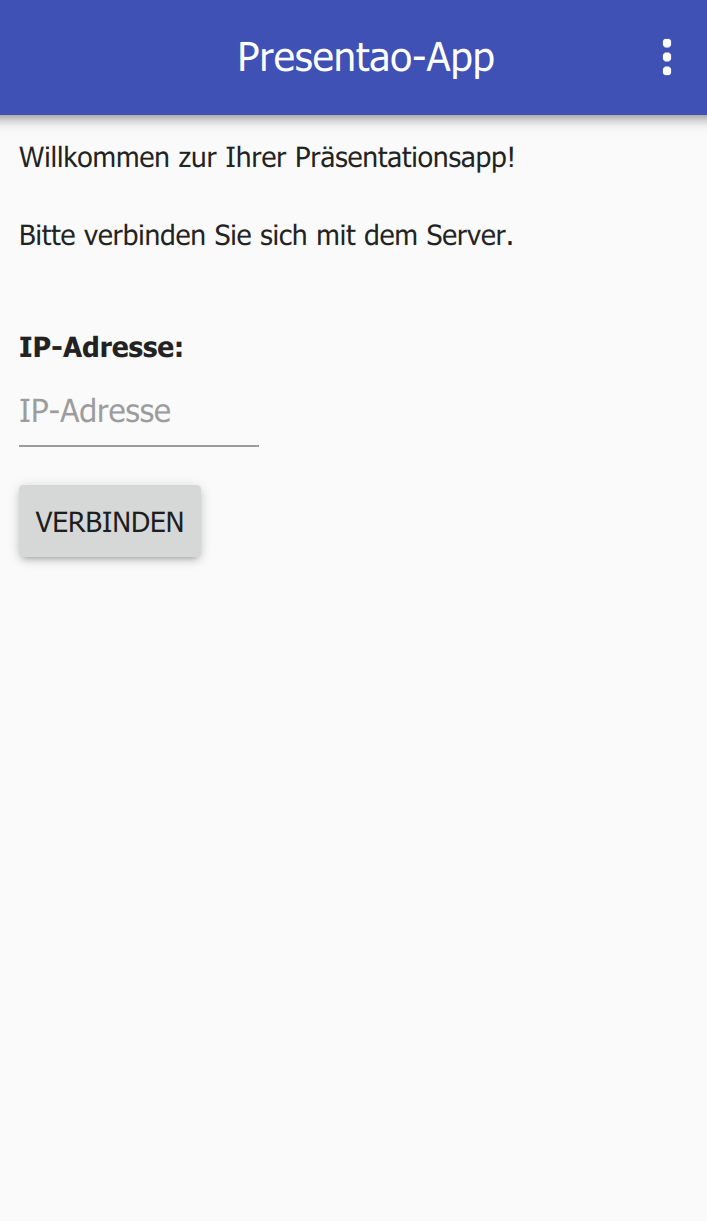
\includegraphics[scale=0.5]{GUI/Bilder/1-Startbildschirm.PNG}
	\end{minipage}
	%\hfill
	\begin{minipage}{0.31\linewidth}
		\centering
		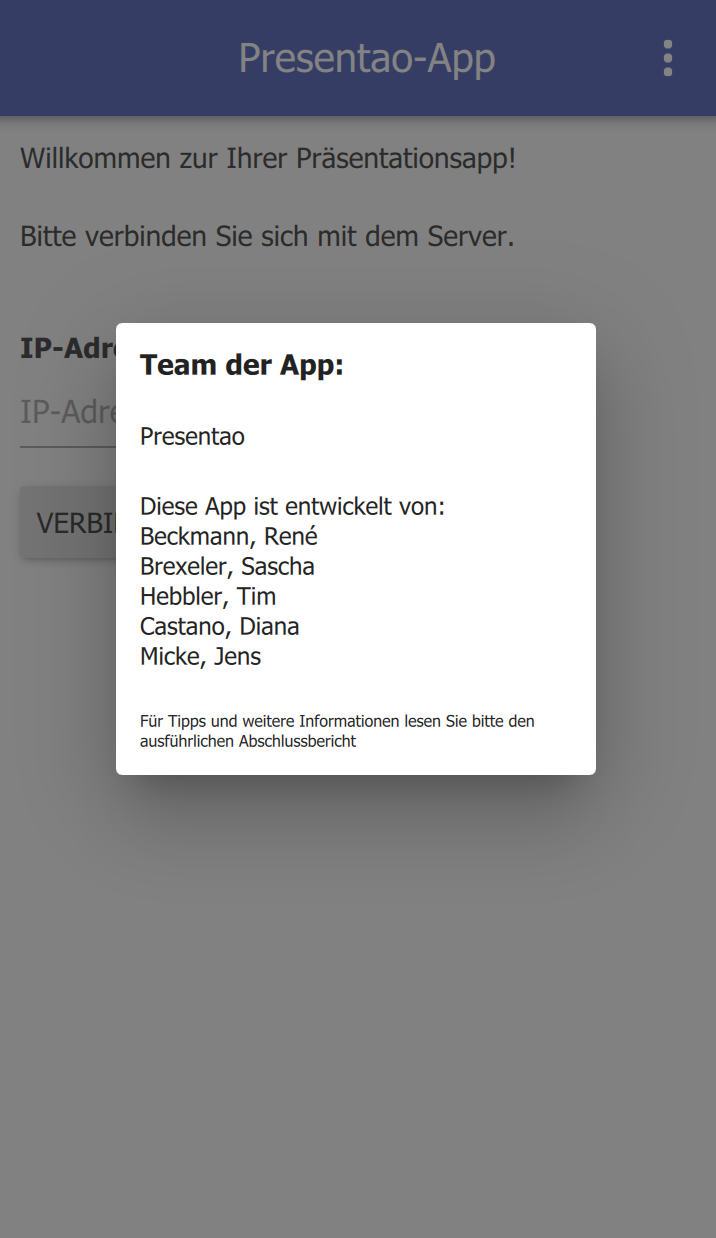
\includegraphics[scale=0.5]{GUI/Bilder/1-0-1-Startbildschirm-PopUP-Team.PNG}
	\end{minipage}
	\begin{minipage}{0.31\linewidth}
		\centering
		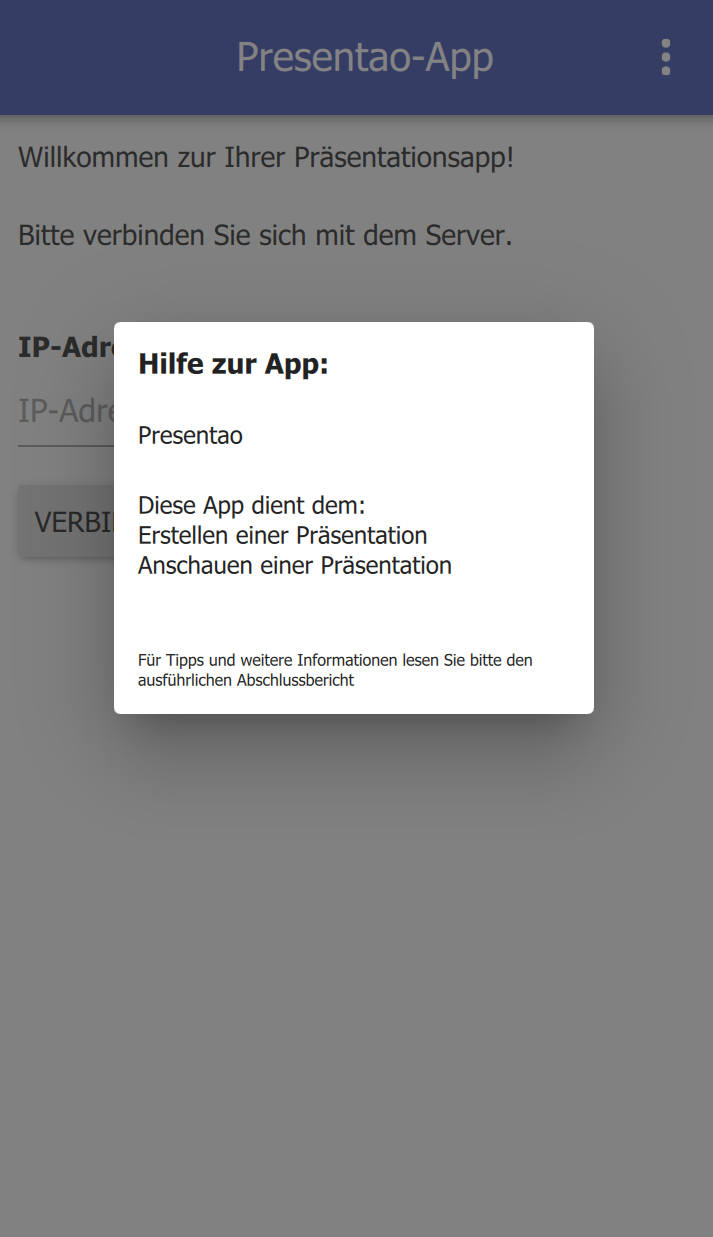
\includegraphics[scale=0.5]{GUI/Bilder/1-0-1-Startbildschirm-PopUP-Hilfe.PNG}
	\end{minipage}
	\caption{v.l.n.r.: Startbildschirm, Über die App, Hilfemenü{\tiny}}
	\label{client:Appstart}
\end{figure}

\newpage

\paragraph{Start der App}$\;$\\
Von dem Startbildschirm aus besteht die Möglichkeit ein Menü (siehe \autoref{client:OptionsMenue}) durch klicken auf den aus drei Punkten bestehenden Menü-Button (siehe \autoref{client:Appstart}) aufzurufen.
\\In diesem lassen sich zwei Pop-Ups zur Hilfe und zum Team aufrufen (siehe \autoref{client:Appstart}).
\begin{figure}[ht!]
	\centering
	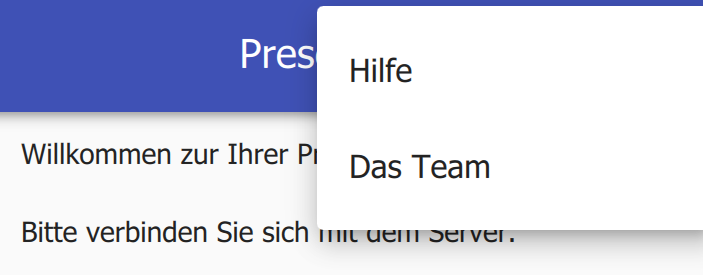
\includegraphics[scale=0.5]{GUI/Bilder/Info-Menu.PNG}
	\caption{Menü{\tiny}}
	\label{client:OptionsMenue}
\end{figure}
\paragraph{Verbindungsaufbau}$\;$\\
Des Weiteren kann der Benutzer nach Eingabe einer der gültigen IP-Adresse eine Verbindung zum Server als Zuhörer aufbauen. Die Eingabe der IP-Adresse erfolgt, wie in der üblichen Notation, mit Punkttrennung und eine Portangabe ist nicht nötig, da diese in Client und Server fest einprogrammiert ist.

\begin{figure}[ht!]
	\centering
	\begin{minipage}{0.31\linewidth}
		\centering
		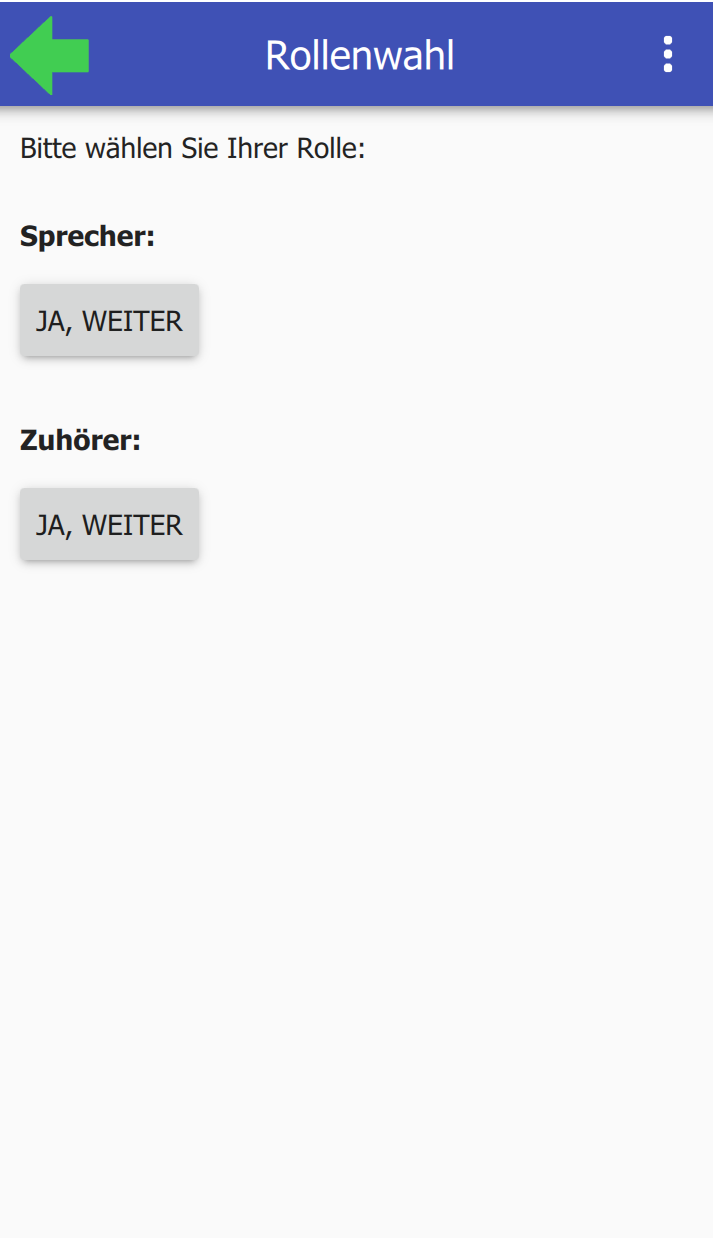
\includegraphics[scale=0.5]{GUI/Bilder/2-Rollenwahl.PNG}
	\end{minipage}
	%\hfill
	\begin{minipage}{0.31\linewidth}
		\centering
		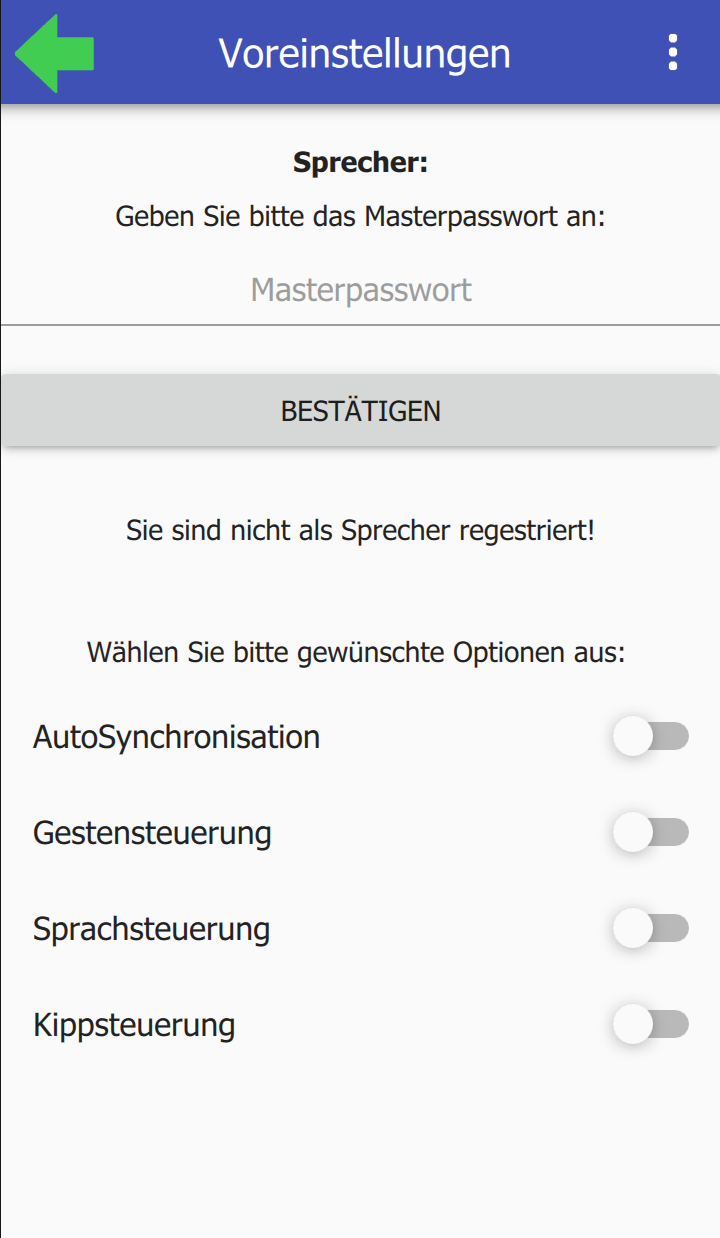
\includegraphics[scale=0.5]{GUI/Bilder/3-S-1-Voreinstellung.PNG}
	\end{minipage}
	\begin{minipage}{0.31\linewidth}
		\centering
		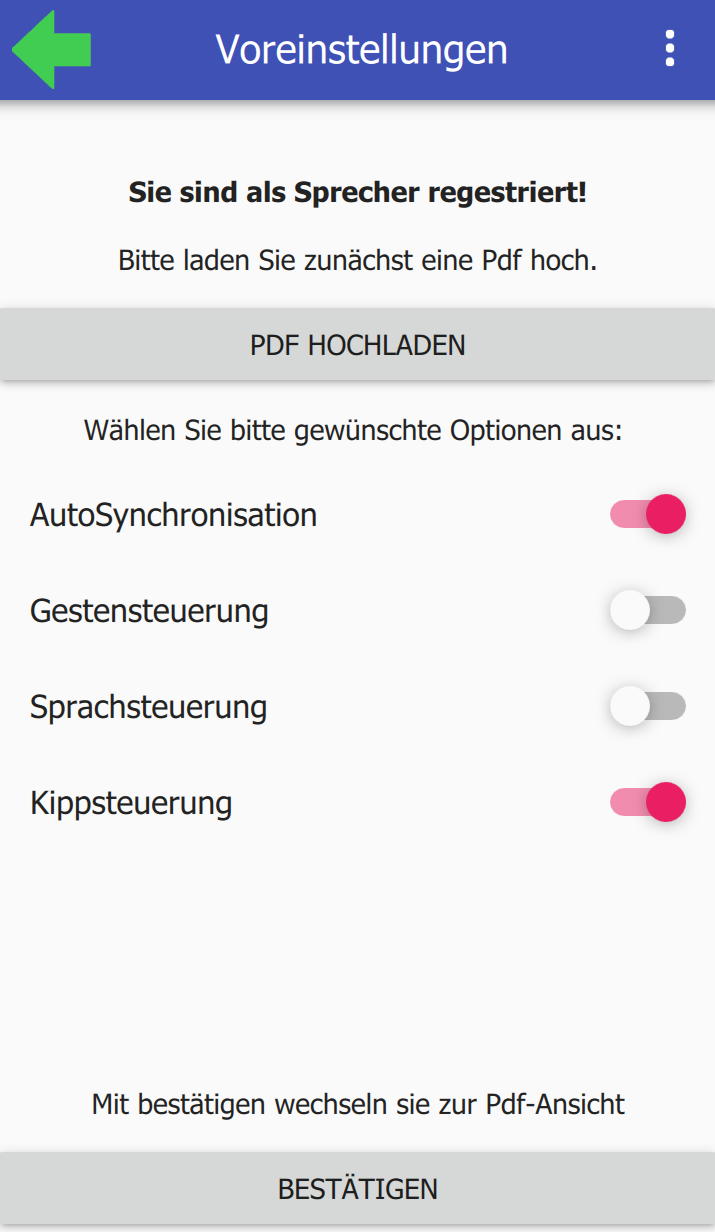
\includegraphics[scale=0.5]{GUI/Bilder/3-S-5-Voreinstellung.PNG}
	\end{minipage}
	\caption{v.l.n.r.: Rollenwahl, Voreinstellungen des Sprecher vor und nach Registrierung{\tiny}}
	\label{client:Rollenauswahl+S-Voreinstellungen}
\end{figure}

\newpage

\paragraph{Auswählen der eigenen Rolle}$\;$\\
Nach erfolgreichen Verbindungsaufbau wechselt die Ansicht in zur Rollenauswahl. Ein Label zeigt diese Position mittig der oberen Leiste (Toolbar) an (siehe \autoref{client:Rollenauswahl+S-Voreinstellungen}).
In dieser Toolbar befindet sich nun zusätzlich ein grüner Pfeil nach links, um zur vorherigen Ansicht zu wechseln.
\\Die Rollenwahl ist wiederholbar und somit korrigierbar, aber unumgänglich implementiert, da weitere Einstellung und Möglichkeiten auf dieser Entscheidung aufbauen.
\paragraph{Voreinstellungen als Sprecher}$\;$\\
Der Sprecher muss sich zunächst als solcher bei dem Server registrieren. Dazu ist eine Passwortabfrage eingerichtet. Das sog. Masterpasswort ist "`mpw12345"'. Wenn die Eingabe fehlerhaft erfolgte, erscheint zusätzlich unter dem Textfeld zur Passworteingabe (siehe \autoref{client:Rollenauswahl+S-Voreinstellungen}) in Dickschrift der Hinweis: "`Bitte überprüfen Sie Ihre Passworteingabe"'. Sobald die Eingabe richtig und bestätigt ist, kann der Benutzer eine Pdf-hochgeladen. Dazu muss der Nutzer eine Pdf-Datei über den File-Dialog (siehe \autoref{client:FileDialog}) suchen und auswählen. Eine Erfolgreiche Auswahl sendet die Datei an den Server, der diese direkt an über den Projektor auf Seite 0 ausgibt. Bevor der Sprecher mit Bestätigen zur Pdf-Ansicht wechselt, sieht dieser noch eine Liste (ListView) mit einige Optionen aus denen er gewünschte über Schiebeschalter (SwitchDelegates) auswählen kann. Mit dem grünen Pfeil wechselt die Ansicht diesmal zurück zur Rollenwahl.

\begin{figure}[ht!]
	\centering
	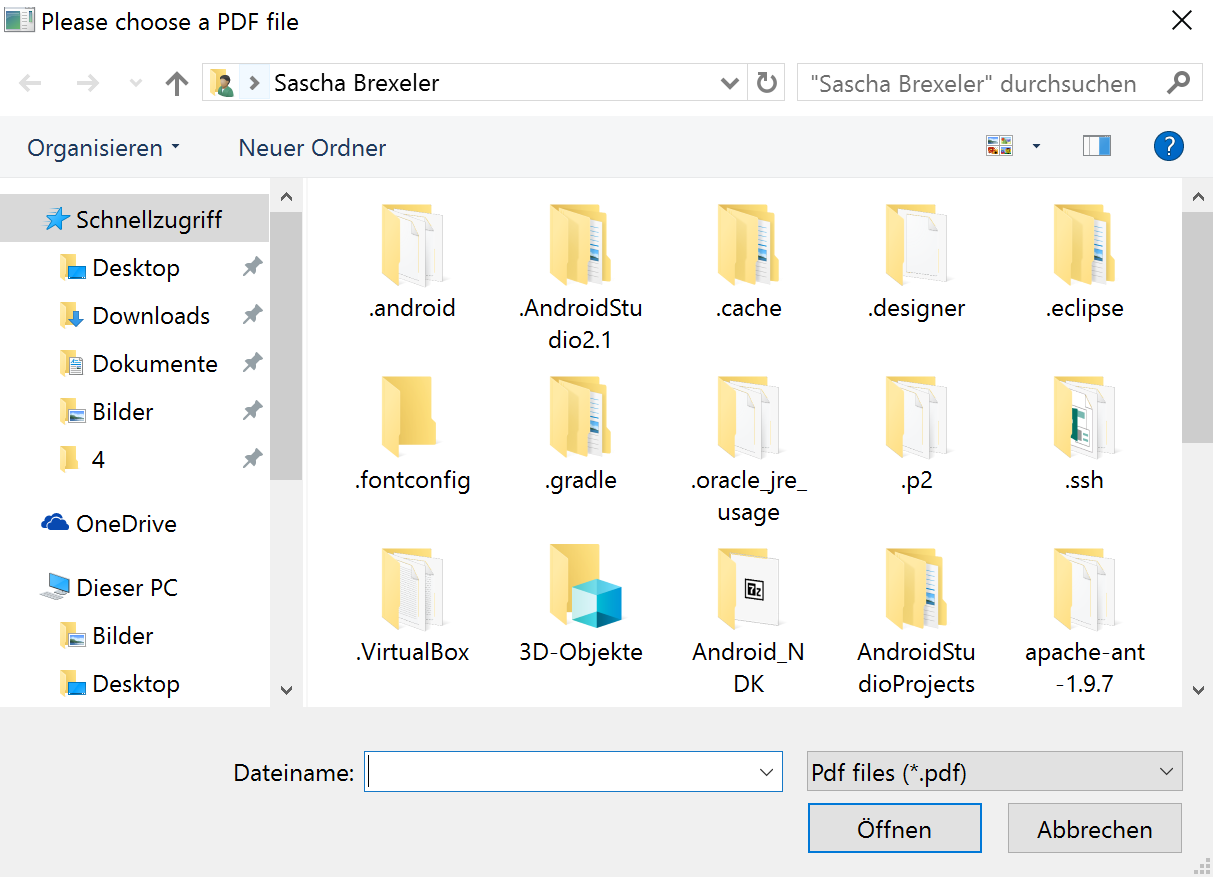
\includegraphics[scale=0.7]{GUI/Bilder/3-S-4-Voreinstellung.PNG}
	\caption{File-Dialog{\tiny}}
	\label{client:FileDialog}
\end{figure}

\begin{figure}[ht!]
	\centering
	\begin{minipage}{0.31\linewidth}
		\centering
		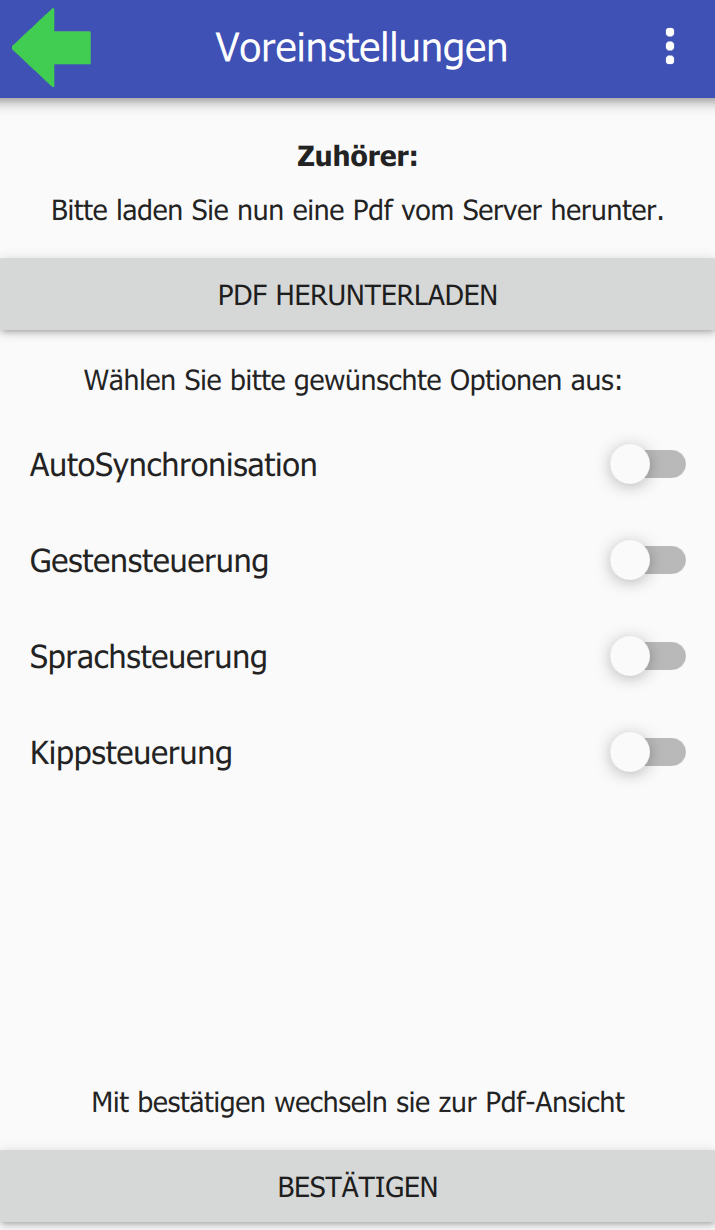
\includegraphics[scale=0.5]{GUI/Bilder/7-H-Voreinstellungen.PNG}
	\end{minipage}
	%\hfill
	\begin{minipage}{0.31\linewidth}
		\centering
		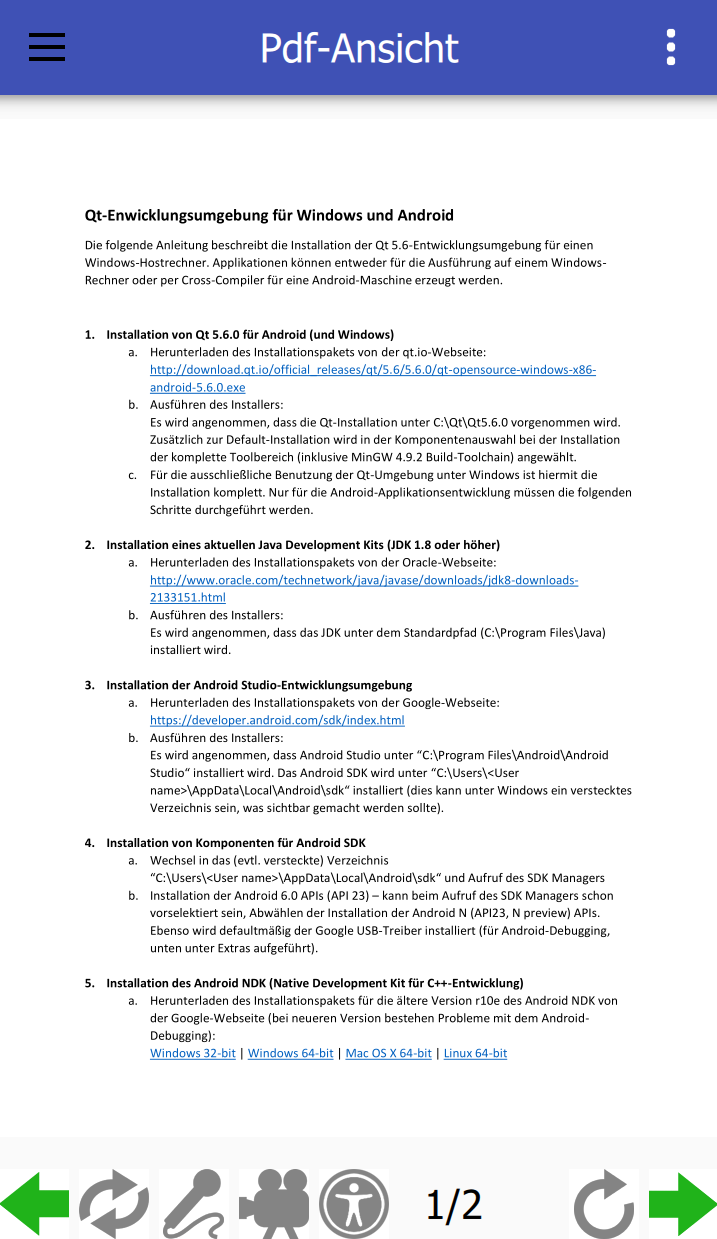
\includegraphics[scale=0.5]{GUI/Bilder/4-S-PDF-Ansicht.PNG}
	\end{minipage}
	\begin{minipage}{0.31\linewidth}
		\centering
		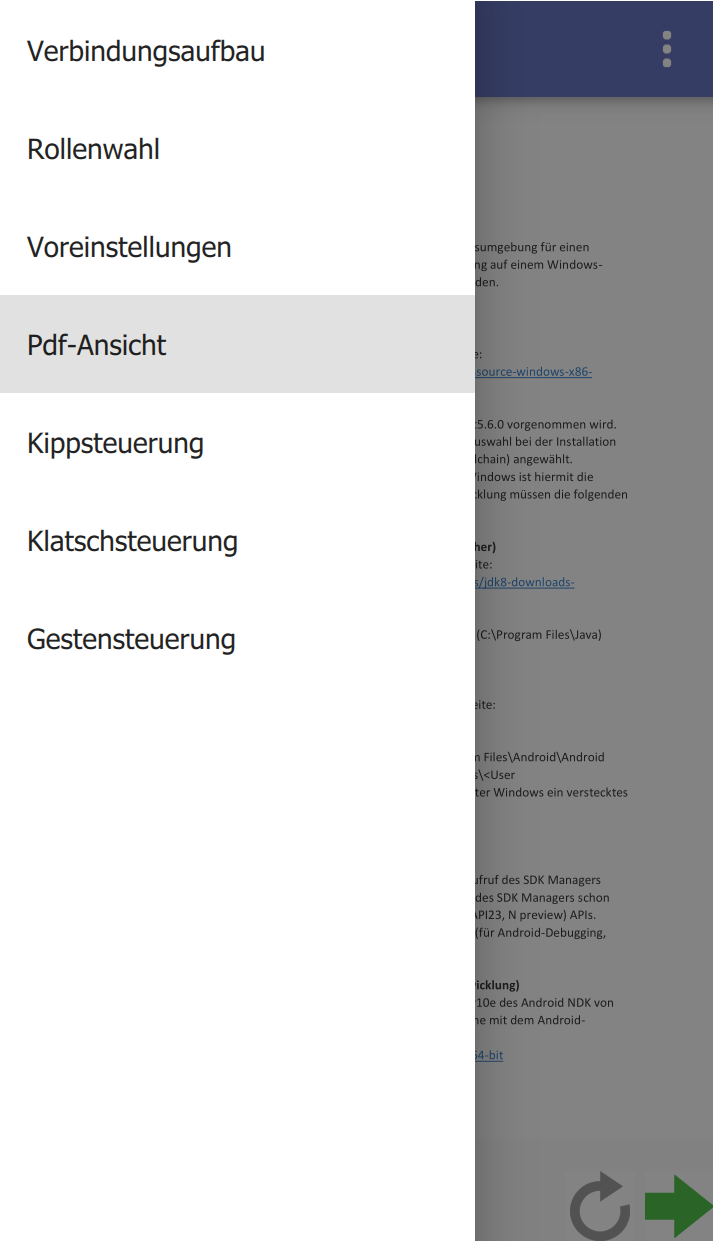
\includegraphics[scale=0.5]{GUI/Bilder/6-Menu-Button-Drawer-mit-Listview.PNG}
	\end{minipage}
	\caption{v.l.n.r.: Voreinstellungen des Zuhörers, PdfAnsicht und Drawer{\tiny}}
	\label{client:H-VoreinstellungenPdfAnsichtDrawer}
\end{figure}

\newpage

\paragraph{Voreinstellungen als Zuhörer}$\;$\\
Als Zuhörer sind die Voreinstellungen ähnlich, jedoch entfällt die Passworteingabe und Herunterladen einer Pdf-Datei ersetzt den Vorgang des Hochladens (siehe \autoref{client:H-VoreinstellungenPdfAnsichtDrawer}). Hierbei erfolgt (ohne eine Auswahlmöglichkeit) das Herunterladen der zuletzt auf dem Server geladenen Datei.
\paragraph{Pdf-Ansicht}$\;$\\
Bestätigen der Voreinstellungen des Sprechers oder Zuhörers bedingt einen Kontextwechsel zur Pdf-Ansicht (siehe \autoref{client:H-VoreinstellungenPdfAnsichtDrawer}).
\paragraph{Drawer}$\;$\\
Ab der Pdf-Ansicht ist der grüne Pfeil oben links durch einen weiteren aus drei waagerechten Strichen bestehenden Menü-Button ersetzt. Dieser Button öffnet eine vertikale Leiste (Drawer) am linken Bildschirmrand, welche ein ListView beinhaltet, dass schnelle Navigation zu allen bisherigen Ansichten und Weiteren ermöglicht (siehe \autoref{client:H-VoreinstellungenPdfAnsichtDrawer}). Durch wischen am vom linken Bildschirmrand nach rechts lässt sich dieser ebenfalls einblenden. Die Navigation über das ListView im Drawer ist nur möglich solange man nicht zu vorherigen Ansichten wechselt. 
\paragraph{Symbolleiste}$\;$\\
Die Pdf-Ansicht beinhaltet ein Symbolleiste (siehe \autoref{client:Symbolleiste}) als Reihe von Icons am unteren Bildschirmrand. Mit ihr ist durch die Pfeile außen ein Blättern in der Pdf möglich. Intuitiv blättert der linke Pfeil zurück, der Rechte vor. Die anderen Buttons dienen dem aktivieren/deaktivieren von Bedienoptionen. Grün signalisiert hierbei aktiviert und grau deaktiviert. Das Mikrofon steht für die Audiosteuerung, das Kamerasymbol für  Gestensteuerung und das Männchen mit den ausgestreckten Armen und Beinen im Kreis für die Kippsteurung. Neben diesem Symbol steht die Seitennummer der angezeigten Seite.
\\Die ineinander greifenden Pfeile signalisieren bei grün, dass die Autosynchronisation aktiv ist. Sobald diese nicht aktiv ist, erscheint ein weiterer Pfeil geschlungen im Uhrzeigersinn in grau auf der Symbolleiste links neben dem Pfeil. Die Funktion ist das manuelle Aktualisieren der Seitenzahl. Ein Sprecher sendet mit dem Refresh-Button die Seitenzahl, die auf seinem Device aktuell ist zum Server, und dieser leitet sie an die Zuhörer-Clients weiter. Ist als Sprecher Autosynchronisation aktiviert, geschieht die bei jedem Blättern automatisch. Zuhörer können über Refresh die aktuelle Seite manuell anfragen oder mit Autosynchronisation alle 2 Sekunden zu der aktuellen Seite zurück springen. Wenn der Sprecher Blättert, erhalten die Zuhörer jedoch in jedem Fall die aktuelle Seite.

\begin{figure}[ht!]
	\centering
	
\includegraphics[scale=0.5]{GUI/Bilder/SchnellLeiste.PNG}
	\caption{Symbolleiste{\tiny}}
	\label{client:Symbolleiste}
\end{figure}

\paragraph{Informationen zur Benutzung}$\;$\\
Da das bisherige Hilfe-Pop-Up nur recht allgemeine Informationen enthält sowie für weitere Hilfestellung auf diese eventuell nicht zur Hand liegenden Dokumentation verweist, kann sich der Benutzer über den Drawer zu einer Erklärung der Bedienmöglichkeiten navigieren. Diese Möglichkeit soll einen möglichst einfachen Einstieg ohne viel ausprobieren sicherstellen und Anwendungsfehler verhindern. Um einen mit dieser Anwendung vertrauten Anwender nicht nach jedem Start durch diese Informationen zu führen, ist das Aufrufen optional (siehe \autoref{client:Symbolleiste}).

\begin{figure}[ht!]
	\centering
	\begin{minipage}{0.31\linewidth}
		\centering
		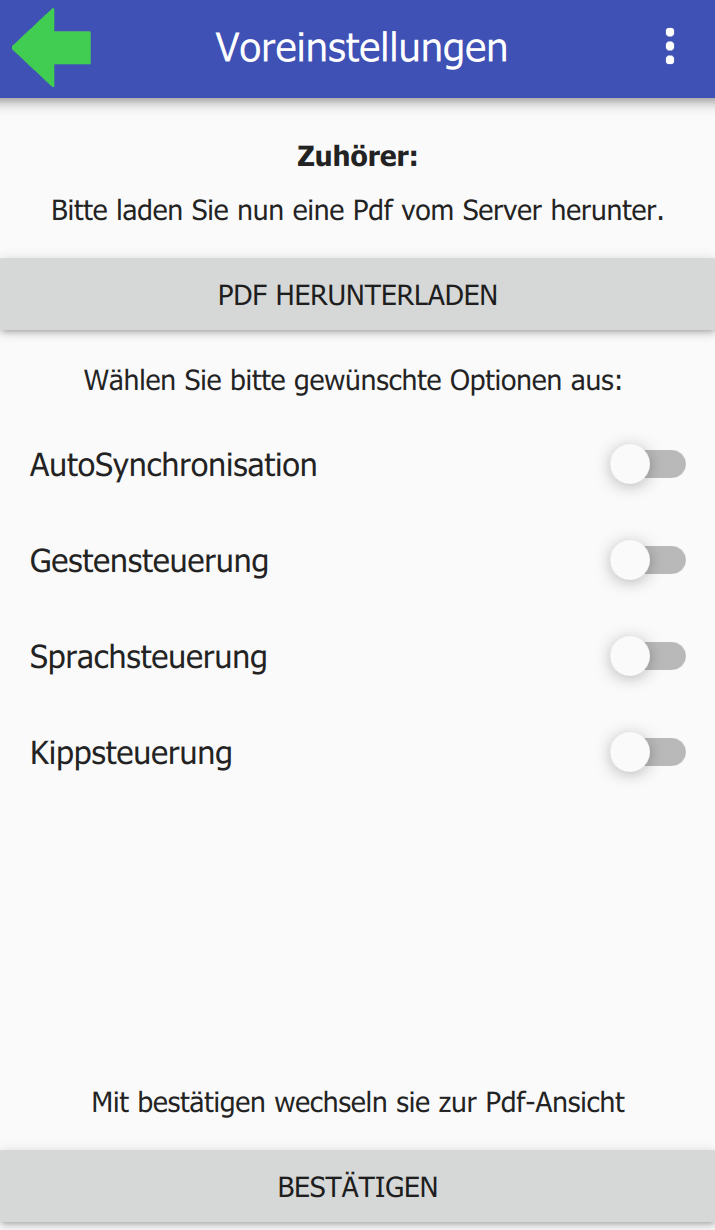
\includegraphics[scale=0.5]{GUI/Bilder/7-H-Voreinstellungen.PNG}
	\end{minipage}
	%\hfill
	\begin{minipage}{0.31\linewidth}
		\centering
		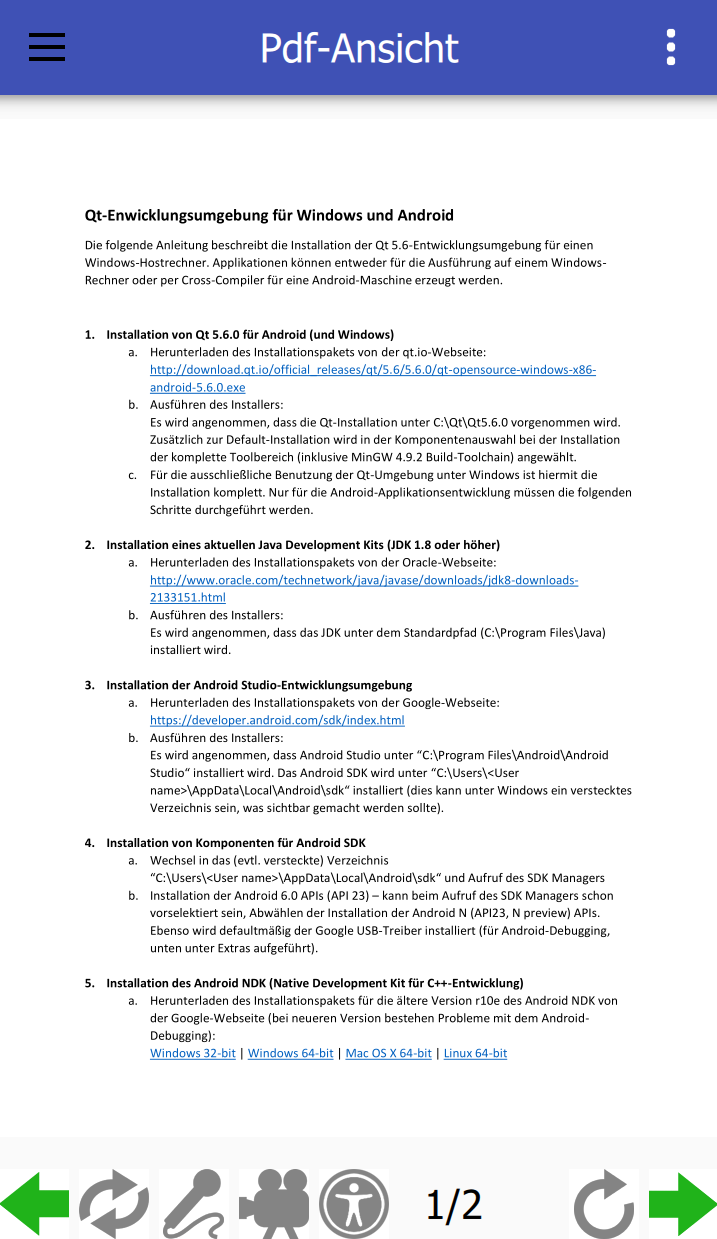
\includegraphics[scale=0.5]{GUI/Bilder/4-S-PDF-Ansicht.PNG}
	\end{minipage}
	\begin{minipage}{0.31\linewidth}
		\centering
		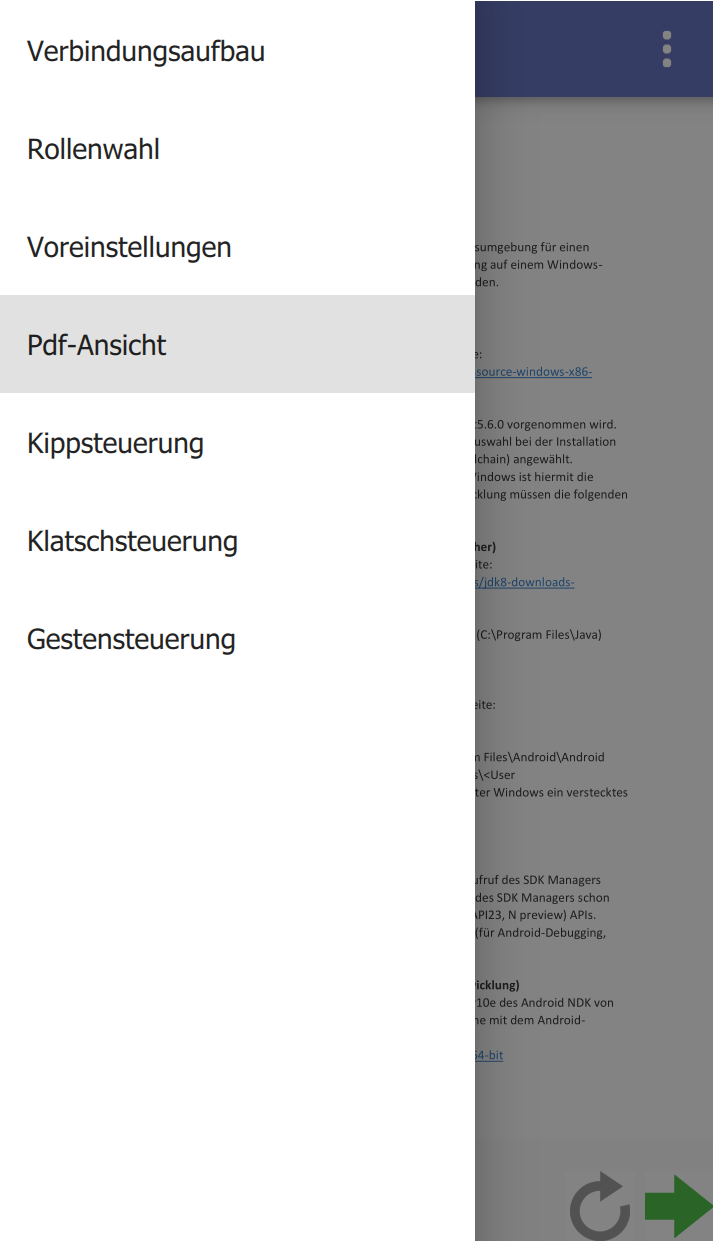
\includegraphics[scale=0.5]{GUI/Bilder/6-Menu-Button-Drawer-mit-Listview.PNG}
	\end{minipage}
	\caption{v.l.n.r.: Gestensteuerung, Kippsteuerung und Klatschsteuerung{\tiny}}
	\label{client:InformationenBedienhilfen}
\end{figure}


\section[Serveranbindung]{Serveranbindung\footnote{Sascha Brexeler}}
\label{client-Serveranbindung}
Die Einbindung der Funktionsblöcke zur Kommunikation des Clients mit dem Server ist in Zusammenarbeit\footnote{zwischen Sascha Brexeler und René Beckmann} im Team entstanden. Hier erfolgt nur eine grobe Beschreibung. Details zur Kommunikation finden Sie in Kapitel ????


\section[Software]{Software\footnote{Sascha Brexeler}}
\label{guiSoftware}
Die Software finden Sie im Git Repository  \footnote{https://github.com/BeckmaR/EmbeddedMultimediaSS2016/tree/master/src/} in im Ordner


\paragraph{Konzept}$\;$\\
Das Softwarekonzept dient der Umsetzung des Bedienkonzepts mit "Qt-Creator"' programmiert in C++ und Qml. Der Qt-Creator ist dafür wegen der Plattformunabhängigkeit ausgewählt.
\paragraph{Struktur}$\;$\\

\paragraph{Zustandssteuerung}$\;$\\
Die Realisierung der Grafische Oberflächen entsprechend bisheriger Einstellungen ist über Zustände einer Variablen "`appState"' realisiert, die sich die aktuellen Einstellungen bzw. den Ort merkt und entsprechend Informationen mittels der Objekteigenschaft "`visible"' ein oder ausblendet.
\paragraph{Elemente}$\;$\\
\paragraph{Einbindung der erweiterten Bedienmöglichkeiten}$\;$\\
\paragraph{Details}$\;$\\
\paragraph{Lektionen}$\;$\\

\section{Navigation}
% !TeX encoding = UTF-8
\chapter{Gestensteuerung}
\thispagestyle{fancy}

Die Gestensteuerung hat die Aufgabe Handbewegungen über eine Smartphone-Kamera zu erkennen. Dabei werden zwei Richtungen erkannt und Signale zum vor- und zurückblättert von PDF-Seiten gesendet. Auf Grund der Vorlesung und Recherchen im Internet war schnell klar, dass \href{http://opencv.org/}{OpenCV} eine zweckmäßige Bibliothek darstellt. Als Qt Basis wurde die Version 5.7 und OpenCV in der Version 3.1 verwendet. Der Code für die Gestenerkennung befindet sich unter folgendem \href{https://github.com/BeckmaR/EmbeddedMultimediaSS2016/tree/master/src/handcontrol}{Link}. Hierbei wurde ein C++ Klasse "`handcontrol"' erstellt, welche in die App eingebunden ist.

\section{Auslesen von Videoframes aus einer Kamera}
Im Laufe des Projektes stellte sich heraus, dass die Einbindung der Kamera, auf den verschiedenen Plattformen Windows und Android, die größte Herausforderung darstellt. Die Windows Unterstützung wurde hauptsächlich ausgewählt, um den Algorithmus nicht umständlich auf einem Android Gerät jedes mal testen zu müssen. Die Implementierung auf der Windows-Plattform war relativ einfach, da OpenCV schon eine Funktion \href{http://docs.opencv.org/3.1.0/d8/dfe/classcv_1_1VideoCapture.html}{VideoCapture} bietet, welche einzelne Videoframes aus eine Kamera auslesen kann und diese in einer Matrix abspeichert. Diese Methode funktionierte leider nicht auf einen Android-Gerät. Hinweise: nachfolgende Funktionsweisen beziehen sich auf den Entwicklungsstand vom 20.7.2016, ggf. sind schon Bugs behoben oder neue Möglichkeiten zur Kameraauswertung hinzugekommen. Vom Autor wurden unterschiedlichste Varianten zum Auslesen der Kamera über mehrere Stunden untersucht. Von Qt werden hauptsächlich \href{http://doc.qt.io/qt-5/videooverview.html}{zwei Möglichkeiten} für das Auslesen eines VideoFrames angeboten. \href{http://doc.qt.io/qt-5/qabstractvideosurface.html}{QAbstractVideoSurface} definiert eine abstrakte C++ Klasse welche die Funktion present() beinhaltet, welcher die einzelnen Videoframes nacheinander übergeben werden. Ähnlich verhält es sich mit \href{http://doc.qt.io/qt-5/qvideoprobe.html}{QVideoProbe} wobei man hier die Verbindung über ein Connect() mit Signal und Slot hergestellt werden muss. Eine weitere Möglichkeit besteht seit Qt 5.5 darin, ein Video Filter\footnote{\label{video_filter}https://blog.qt.io/blog/2015/03/20/introducing-video-filters-in-qt-multimedia/} in QML zu verwenden und mit Hilfe der Klasse \href{http://doc.qt.io/qt-5/qabstractvideofilter.html}{QAbstractVideoFilter} die einzelnen Videoframes in C++ zu analysieren und ggf. wieder nach QML zu transformieren. Die C++ QCamera funktioniert nicht auf Android-Geräten (\href{https://bugreports.qt.io/browse/QTBUG-41194}{1},\href{http://stackoverflow.com/questions/28041741/qt-qml-camera-to-c-qimage-on-android}{2}), sodass auf das in QML integrierte Camera Objekt zurückgegriffen wird. Bei der QAbstractVideoFiler Variante konnten die Videodaten in Android nicht in den CPU-Adressraum gemappt werden. Mit QVideoProbe war dies möglich. Hierbei wird aus QML das QCamera Objekt in C++ adressierbar gemacht und mit dem QVideoProbe verbunden. Seit Qt 5.6 existiert ein VideoOutput Objekt in QML welches das Auslesen und Anzeigen von VideoFrames steuert, sodass das hier angegebene \href{http://stackoverflow.com/questions/28041741/qt-qml-camera-to-c-qimage-on-android/33238150\#33238150}{Beispiel} noch um ein VideoOutput Objekt ergänzt werden muss. Um keine größeren Unterschiede zwischen dem Algorithmus für die Windows- und der Androidversion zu haben, ist es wünschenswert beide Cameras über Qt auslesen zu lassen. Leider funktioniert der oben für Android vorgestellte Ansatz für Windows nicht. Hier ist ein Workaround mit einer C++ QCamera und dem QAbstractVideoSurface nötig, um ein QVideoFrame zu erhalten. Die neue Variante mit dem "`Video Filter"' wurde auch untersucht, hat aber nur auf ein paar Androidgeräten funktioniert \href{https://bugreports.qt.io/browse/QTBUG-47934/}{QTBUG-47934}. Anscheinend gibt es dort noch Fehler in dem Qt-Framework. Unter folgendem \href{https://wiki.qt.io/Qt_5.7_Multimedia_Backends}{Link} gibt es eine Auflistung welche Funktionen in dem Qt-Multimedia-Framework-5.7 auf den verschiedenen Plattformen aktuell funktionieren.

\subsection{Verbesserungen}
Die mit Qt 5.5 eingeführten Video Filter scheinen ein gute Weg zu sein, um VideoFrames in Qt analysieren zu können. Leider ist aktuell die Implementierung nicht auf allen Androidgeräten funktional, sodass auf ein Workaround mit QVideoProbe zurückgegriffen werden musste. Diese Variante ist aber leider nicht optimal, da sie Verzögerungen zwischen dem Aufnehmen und dem Aufruf der Funktion present() enthält\footnote{https://blog.qt.io/blog/2015/03/20/introducing-video-filters-in-qt-multimedia/\#comment-1195419}. Eine weitere Möglichkeit besteht, QML \href{http://doc.qt.io/qt-5/qml-qtquick-shadereffect.html}{ShaderEffect} mit OpenGL zu verwenden. Da die Android Kamera seine Videoframes auf der Grafikkarte in OpenGL Texture vorhält \footnote{https://blog.qt.io/blog/2015/03/20/introducing-video-filters-in-qt-multimedia/\#comment-1195414}, wäre es sinnvoll diese auch dort weiter zu verarbeiten. Das kann seit neuem mit Video Shader Objekten direkt in QML programmiert werden. Außerdem war es dem Autor über QML nicht möglich exakte Auflösungen und Frameraten einzustellen. Anscheinend ignoriert Qt gewisse Parameter auf verschiedenen Platformen oder es stehen nicht alle Einstellung zur Verfügung. Jedenfalls sind diese nicht richtig dokumentiert. Ein Problem ist außerdem, dass es vorkommen kann das Frameraten von 30 fps auf 16 fps einbrechen oder kein reproduzierbares Verhalten zeigen. Dieser Punkt konnte innerhalb der Arbeit leider nicht geklärt werden. Eine andere Möglichkeit, welche nicht weiter verfolgt wurde, wäre über Qt mit den \href{http://doc.qt.io/qt-5/qtandroidextras-module.html}{Qt Android Extras} die Androidkamera über Java Code in die Qt Anwendung einzubetten, ggf. auch über das vorhandene OpenCV Java Binding. 

\section{Handerkennungsalgorithmus}
Aus Qt liegen die QVideoFrames als RGB (Windows) und als YUV420 (Android) vor. Diese werden als erstes in Grauwertbilder umgewandelt. Bei dem Android QVideoFrame muss keine pixelweise Konvertierung durchgeführt werden, sondern es wird nur der Luminanz Y Teil des Bildes genommen. Anschließend wird das Differenzbild zwischen dem aktuellen und vorherigen Grauwertbild berechnet. Hierbei achtet OpenCV selbständig darauf, dass eine Sättigung im Zahlenbereich durchgeführt wird.

\begin{figure}[ht!]
\centering
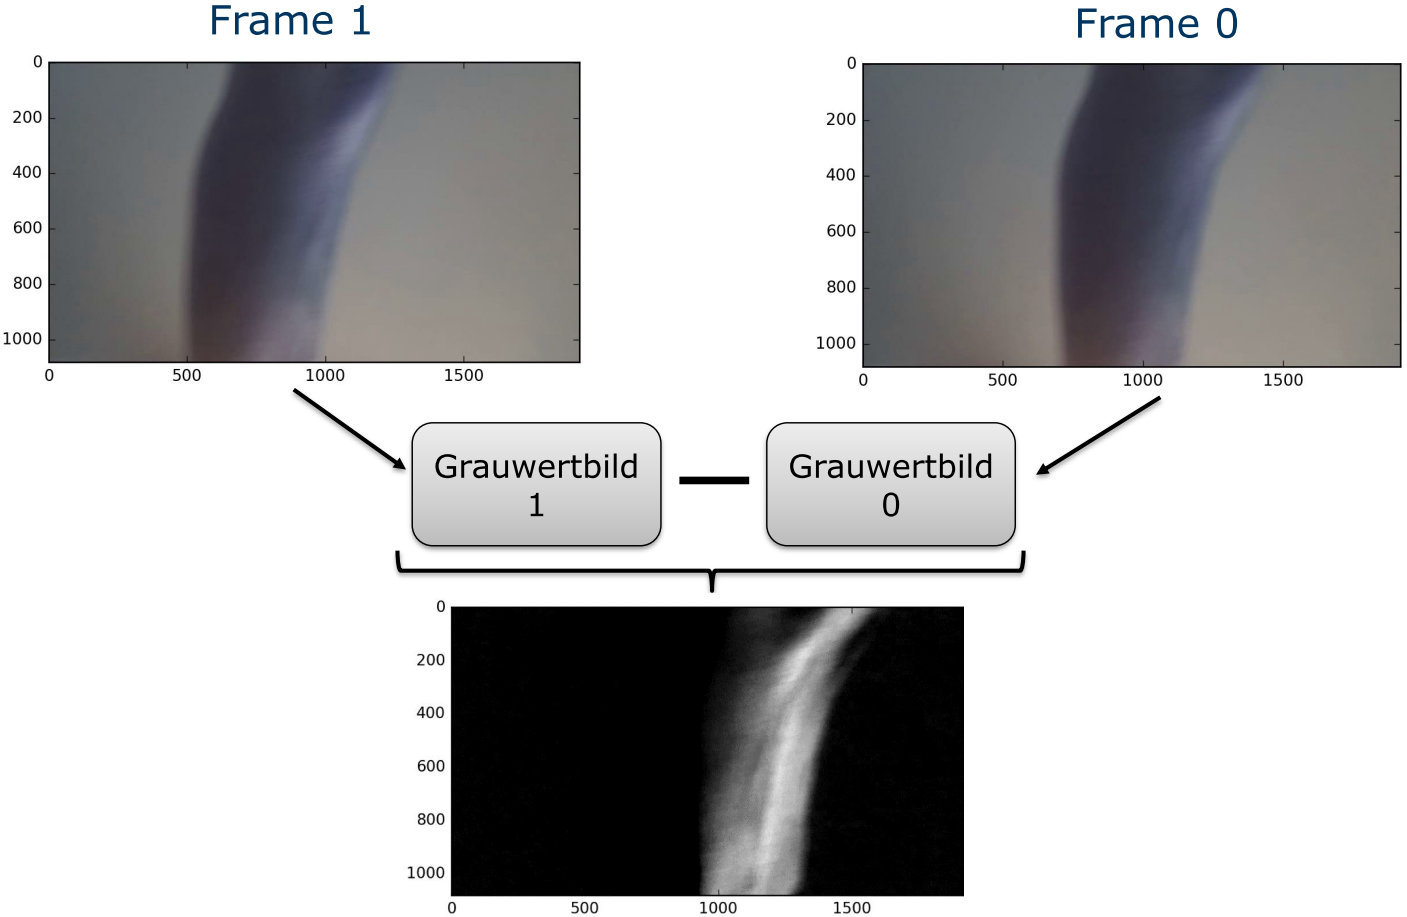
\includegraphics[angle=0,width=14cm]{handcontrol/Bilder/diff_frame1-frame0.png}
\caption{Differenzberechnung zwischen aktuellem und vorherigen Grauwertbild}
\end{figure}

Im nachfolgenden Schritt wir mit Hilfe der reduce() Funktion von OpenCV ein Mittelwert über alle Spalten gebildet. Man erhält einen Zeilenvektor wobei jeder Eintrag den Mittelwert eine Spalte repräsentiert. Hierbei kann man schnell erkennen wo sich in der Horizontalen die größten Änderungen ergeben. Das nennt der Autor Histogramm, da es die Häufigkeitsverteilung darstellt.

\begin{figure}[ht!]
\centering
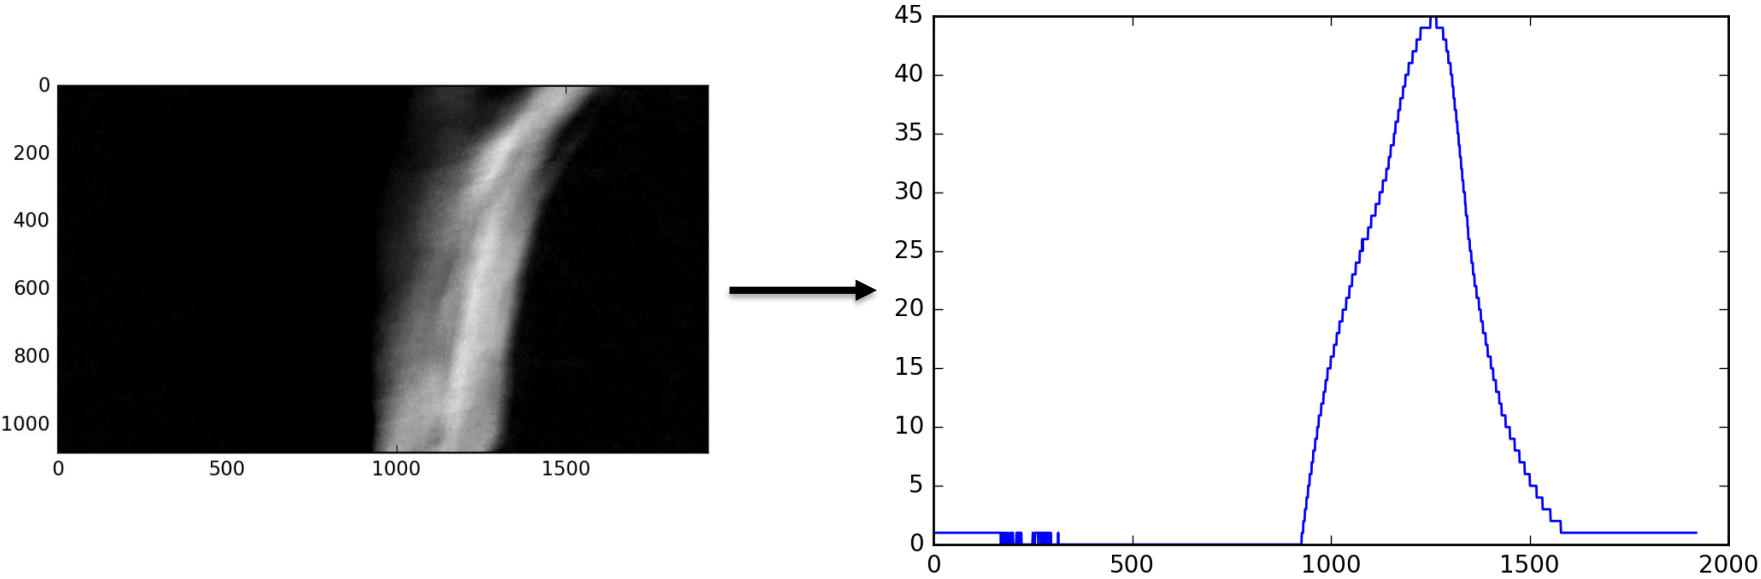
\includegraphics[angle=0,width=14cm]{handcontrol/Bilder/diff_frame_to_hist.png}
\caption{Berechnung des Histogramms über die Spalten eines Differenzbildes}
\end{figure}

Untersucht man die Verschiebung des Histogramms über die Horizontalen, kann man Handbewegungen erkennen. Hierbei wird als erstes der Schwerpunkt des Histogramms gebildet. Das geschieht mit Hilfe einer kumulierten Summe über alle Histogrammwerte. Würde man nur den maximalen Wert des Histogramms betrachten, kann bei verrauschten Bildern eine zu große Abweichung auftreten. Vor dem Berechnen des Schwerpunktes wird noch ein konstanter Faktor subtrahiert, um den ggf. existierenden Rauschteppich zu entfernen. Zur weiteren Fehlerreduktion wurden im folgenden nur diese Schwerpunkte ausgewählt, welche auch mindestens einen gewissen maximalen Histogrammwert aufweisen. Der Wert kann im Sourcecode nachgelesen werden. Um auszuwerten, ob eine PDF vor- oder zurückgeblättert werden soll, untersucht der Algorithmus zeitlich aufeinanderfolgende Schwerpunkte von Histogrammen der Differenzbilder. Er sendet ein Signal, wenn ohne Unterbrechung der Schwerpunkt eine gewisse Zeit in eine der beiden Richtungen gewandert ist. Um den GUI-Thread nicht zu überlasten und um eine flüssige Bedienung der GUI sicher zu stellen, wurde der Algorithmus in ein QThread verschoben. Der so beschriebene Algorithmus benötigt mit 30 Frames pro Sekunde auf Windows ~7ms und auf Android ~10 ms. Somit ist die Echtzeitfähigkeit gegeben. Als Alternative zum dem Differenzbild wurde auch der in OpenCV implementierte Background Substraction Algorithmus (\href{http://docs.opencv.org/3.0-rc1/d7/d7b/classcv_1_1BackgroundSubtractorMOG2.html}{BackgroundSubtractorMOG2}) untersucht. Dieser schätzt den Hintergrund über gaußsche Mischungsverhältnisse mit Mittelwert und Kovarianzmatrix. Leider benötigt der Algorithmus viel Berechnungszeit (~14 Windows und ~30 ms Android) und kratzt somit bei Android Geräten an der Echtzeitfähigkeit. Außerdem würde eine solche Implementierung zu viel Energie des Akkus verbrauchen und wurde deshalb verworfen.

\begin{figure}[ht!]
\centering
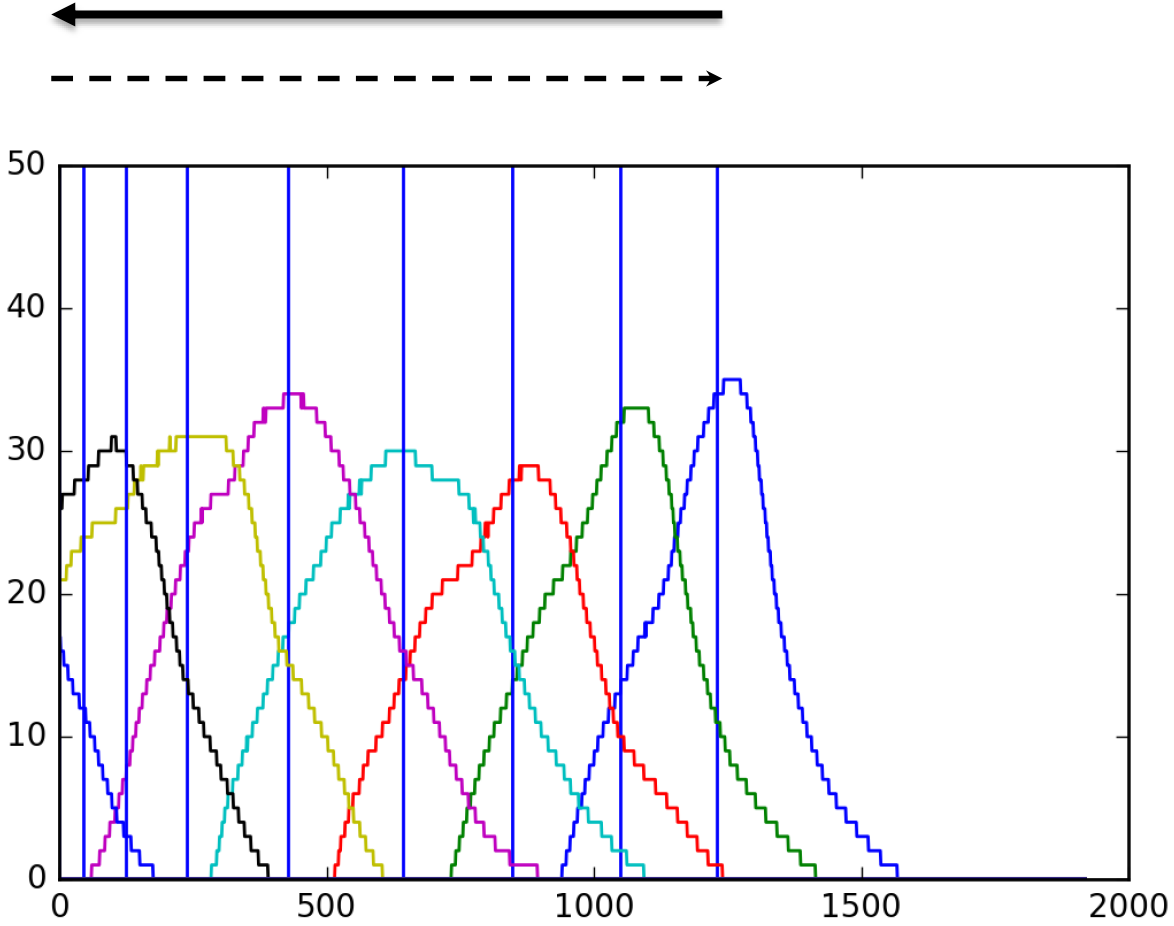
\includegraphics[angle=0,width=14cm]{handcontrol/Bilder/histogramm_schwerpunkt.png}
\caption{Histogramme der Differenzbilder mit Schwerpunkt}
\end{figure}

\section{Entwicklung des Algorithmus}
Der Algorithmus wurde als erstes in MATLAB mit aufgenommenen Videos entwickelt. Nachher wurde auf Python mit OpenCV Binding umgestellt, um einen besseren Vergleich mit der C++ Version zu gewährleisten. Als IDE für Python wurde \href{https://github.com/spyder-ide/spyder}{Spyder} mit dem \href{https://www.continuum.io/downloads}{Anaconda Framework} verwendet. Um den Algorithmus separat von der App zu entwickeln wurde ein "`test\_handcontrol.pro"' Projekt erstellt, welches als eine Art Modultest fungiert. Zu finden in dem schon am Anfang des Kapitels genannten Verzeichnis in Github.

\section{Verbesserungen}
Die Verbesserungen zum Auslesen der Kamera wurden schon in einem separaten Abschnitt behandelt. Für den Algorithmus könnte man statt Grauwertbilder auch Bilder aus dem HSV Raum verwenden. Dort könnte man ggf. Helligkeitsveränderung besser abfangen. Außerdem kann es manchmal vorkommen, dass mehrfach Erkennung erfolgen, diese könnten durch einen Timer abgefangen werden. Eine Verschiebung der Berechnung zur Grafikkarte mittels OpenGL oder OpenCL, wie vorher schon erwähnt, könnte die CPU entlasten und ganz andere Möglichkeiten der Analyse des Frames bieten. Bei der Differenzbildung der Frames entstehen positive und negative Abweichungen, diese könnten in einem verbesserten Algo. separat berücksichtigt werden.

Beschleunigungssensor}

\section{Features}
- Blättern in einer Pdf ohne dass ein Update auf dem Server erfolgt\\
\\INOF ans TEAM:Diese Section ist noch nicht fertig
\section{Erweiterungspotential}
Einige zusätzliche Funktionalitäten könnten, den Wert der Applikation für Zuhörer und Sprecher steigern.\\
\\INOF ans TEAM:Diese Section lade ich später hoch
\\INOF ans TEAM:Wenn Ihr die Zuverlässigkeit der Gestensteuerung, Kippsteuerung, Audiosteuerung oder die Sicherheit der Kommunikation noch verbessern wollt, könnt ihr ja wie Tim es in euren Abschnitt einfügen. Hier geht es nur um Erweiterungen der allgemeinen mögliche Funktionalität der Clientapp wie Puplikumsfragen oder sowas.
Erweiterungen für den Sprecher:\\

Erweiterungen für den Zuhörer:\\
- Einstellen der Zeit die vergehen soll bis sich die Applikation synchronisiert\\






\newpage
So kann Code eingefügt werden.
\begin{lstlisting}[frame=single,breaklines=true,basicstyle=\tiny,language=C,label={PWMStart},caption={Kommentierter Start der PWM}]
/*! \brief Starts the PWM
* 
* To make sure that the PWM behaves correctly after a Compare Bit Change the PWM is started and reset with a software trigger.
*/
static void vStartPwm( void )
{
tc_start( &AVR32_TC0, PWM_CHANNEL );
tc_software_trigger( &AVR32_TC0, PWM_CHANNEL );
}
\end{lstlisting}